\chapter{Espionaje en red WPA2-PSK}
A continuación, veremos cómo podemos obtener las credenciales de un usuario que inserte sus datos en una página web con protocolo HTTP.

Para ello usaremos un ordenador con sistema operativo GNU/Linux como puede ser Debian, Ubuntu, Kali Linux, etc.

\Nota De las dos versiones de WPA2 existentes, nos centraremos en WPA2-PSK para la práctica.
\section{Conocemos la passphrase}
Cuando conocemos la passphrase, podemos dirigirnos a la señal Wi-Fi del AP al cual queremos conectarnos e introducirla manualmente como un usuario normal y estaremos dentro de la red.

Con la finalidad de obtener las credenciales de un usuario, debemos prepararnos para un ataque Man-in-the-Middle\footnote{Un ataque Man in-the-Middle es aquel en el que se un atacante adquiere la capacidad de leer, insertar y/o modificar a voluntad propia el contenido de los paquetes enviados por una víctima y capturados por dicho atacante.}, que usaremos para obtener los datos.

\subsection{Instalación de Ettercap}
Ettercap es un sniffer que hace posible la inyección de datos en una conexión establecida y filtrado al vuelo aun manteniendo la conexión sincronizada, lo que nos permitirá recrear un ataque Man-in-the-Middle.

Para instalar ettercap en modo gráfico deberemos seguir los siguientes pasos:
\begin{enumerate}
	\item Nos dirigimos a la terminal e introducimos los siguientes comandos para instalar los paquetes previos:
	\begin{center}
		\texttt{sudo apt-get install zlib1g zlib1g-dev}
		%Aprovechar el center para la foto
		
		\texttt{sudo apt-get install build-essential}
		%Aprovechar el center para la foto
		
	\end{center}
	\item A continuación introducimos el siguiente comando para instalar ettercap en modo gráfico:
	\begin{center}
		\texttt{sudo apt-get install ettercap-graphical}
		%Aprovechar este center para poner la foto del comando.
		
	\end{center}
	\item Abrimos Ettercap en modo gráfico con el siguiente comando:
	\begin{center}
		\texttt{sudo ettercap -G}
		%Aprovechar este center para poner la foto del comando y del ettercap abierto.
		
	\end{center}
\end{enumerate}

\Nota Si estamos usando Kali Linux (o algún otro sistema operativo para la seguridad y hacking ético) debemos tener en cuenta que puede venir instalado por defecto.

\subsection{Preparación del ataque}
Ya tenemos todo lo necesario en nuestro ordenador para reproducir el ataque con éxito. Solo nos queda preparar el ataque y que nuestra víctima acceda a una página web con protocolo HTTP.

\subsubsection{ARP Poisoning}
Un ARP Poisoning es un ataque en el que el atacante envía mensajes ARP falsos al AP. Como resultado de este ataque la dirección ARP del atacante queda vinculada a la dirección ARP del AP.

Veamos lo que ocurre paso a paso:
\begin{enumerate}
	\item El atacante envía un ARP replay para envenenar la tabla ARP de la víctima.
	\begin{center}
		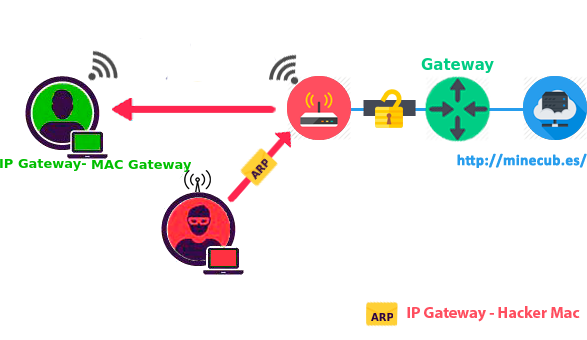
\includegraphics[scale=0.7]{ARPpoison1.png}
	\end{center}
\newpage
	\item La víctima modifica su tabla ARP relacionando la IP de la puerta de enlace con la MAC del atacante.
	\begin{center}
		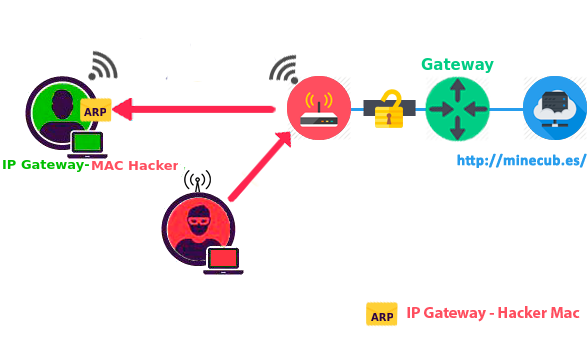
\includegraphics[scale=0.7]{ARPpoison2.png}
	\end{center}
\end{enumerate}

Hasta aquí quedaría configurado el ARP Poisoning. Por lo tanto, cuando el usuario quiere acceder a algún servicio web ocurre lo siguiente:
\begin{enumerate}
	\item La víctima lanza una solicitud HTTP.
	\begin{center}
		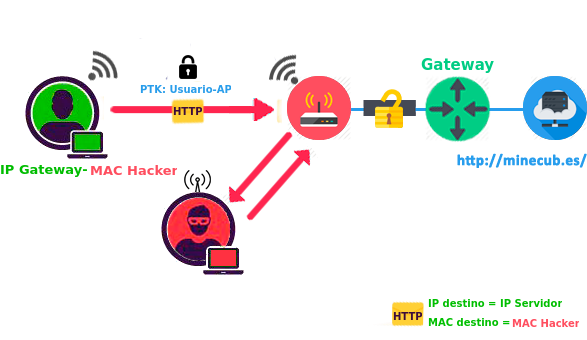
\includegraphics[scale=0.7]{ARPpoison3.png}
	\end{center}
\newpage
	\item El AP redirecciona el paquete a la MAC del atacante.
	\begin{center}
		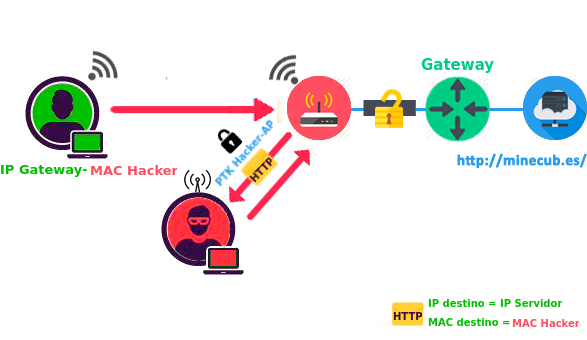
\includegraphics[scale=0.7]{ARPpoison3-2.png}
	\end{center}
	\item El atacante lee y envía el paquete al destinatario legítimo sin que la víctima sea consciente de ello.
	\begin{center}
		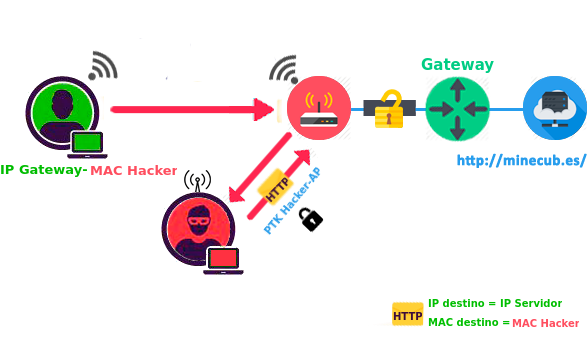
\includegraphics[scale=0.7]{ARPpoison3-3.png}
	\end{center}
\end{enumerate}
\newpage
Por lo tanto, el escenario resultante después de la configuración del ARP Poisoning es el siguiente:
\begin{center}
	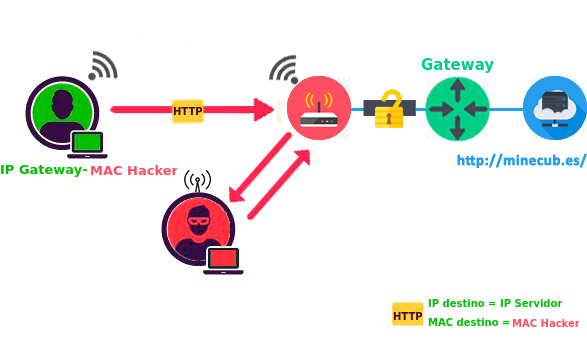
\includegraphics[scale=0.7]{Escenario.png}
\end{center}

\Nota En estos ejemplos se ha usado la página web \url{http://minecub.es/} por tener protoclo HTTP.

\Nota En caso de que la red sea abierta (sin contraseña) el procedimiento es exáctamente igual una vez que estamos conectados a la red.

\subsubsection{HTTPS}
HTTPS es una protocolo de aplicación basado en HTTP y destinado a la transferencia segura de paquetes HTTP, es decir, es al versión segura de HTTP.

HTTPS utiliza un cifrado basado en SSL/TLS para crear un canal cifrado (cuyo nivel de cifrado depende del servidor remoto y del navegador utilizado por el cliente). De este modo se consigue que la información sensible no pueda se r usada por un atacante que haya conseguido interceptar la transferencia de datos de la conexión, ya que lo único que obtendrá seerá un flujo de datos cifrados que le resultará imposible de descifrar.

Por ello, para poder obtener las credenciales de usuario, se ha insistido tanto en que la web a la que acceda la vícitma tendrá que tener protocolo HTTP.

\section{No conocemos la passphrase}
Hasta hace poco, en el caso de no conocer la passphrase de la red Wi-Fi, no podríamos acceder a ella a no ser que usáramos un ataque de fuerza bruta o de diccionario. Pero a partir del 16 de octubre de 2017 contamos con una nueva herramienta que nos permite entrar a una red Wi-Fi sin necesidad de conocer la passphrase.

\subsection{KRACK}
Key Reinstallation AttaCK: Es un ataque que se basa en forzar el reuso del SNonce del saludo de cuatro vías de WPA2-PSK, de tal forma que se puedan desencriptar los datos. Por lo que no es necesario el conocimiento de la passphrase de la red.

El saludo de cuatro vías de WPA2-PSK es el siguiente:
\begin{center}
	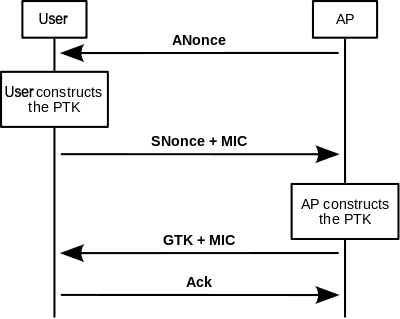
\includegraphics[scale=0.7]{Saludo4vias.png}
\end{center}
Tal como se puede ver en la imagen, una vez que el AP envía su ANonce al usuario y este construye la PTK, envía al AP su SNonce.

Es en ese envío del SNonce donde ataca KRACK haciendo que se reenvíe dicho SNonce hasta uno conocido por el atacante lo que nos permitirá pertenecer a la red sin necesidad de la passphrase y podremos espiar (tal como hemos hecho en las redes donde sí conocíamos la passphrase a los usuarios).

\subsubsection{Recursos para usar KRACK}
Para realizar el ataque KRACK nos harán falta los siguientes recursos:
\begin{itemize}
	\item Rogue-AP: Es un punto de acceso que tiene por objetivo que los usuarios se conecten a el para, una vez dentro, capturar su tráfico.
	\item Man-in-the-Middle.
	\item Script KRACK\footnote{Este script fue creado por el descubridor de KRACK y no ha sido publicado en la web debido a que dicha persona (Mathy Vanhoef, estudiante en criptografía) lo comunicó directamente a la Wi-Fi Alliance que se puso manos a la obra en la creación del nuevo protocolo de seguridad, WPA3 que veremos en un futuro en funcionamiento.}.
	\item SSLStrip: Es una applicación capaz de ``descifrar el trágico HTTPS'' que viaja a través de una red\footnote{Realmente SSLStrip no desencripta todo el tráfico HTTPS sino que solo es capaz de engañar al servidor cuando la víctima llegaa la web mediante una redirección o un link.}.
	\item Un sniffer: Por ejemplo Wireshark.
\end{itemize}